\documentclass[border=16pt]{standalone}
\usepackage{amsmath}
\usepackage{tikz}
\usetikzlibrary{arrows.meta, positioning, fit, backgrounds, calc}

\begin{document}
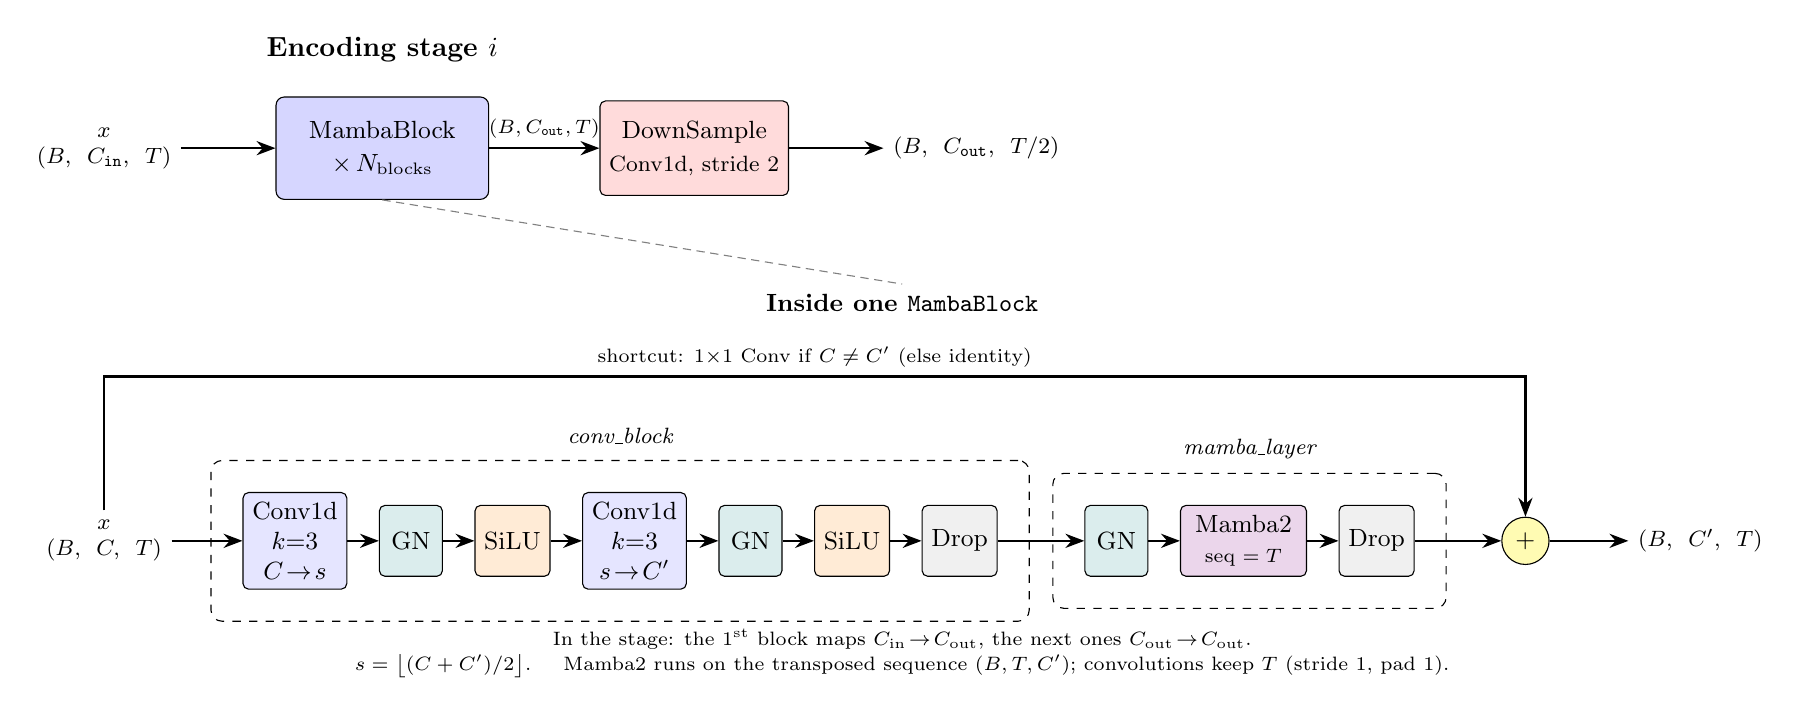
\begin{tikzpicture}[
    font=\small,
    >={Stealth[length=2.4mm]},
    io/.style   = {align=center, font=\ttfamily\footnotesize},
    conv/.style = {draw, rounded corners=2pt, align=center, minimum height=9mm,
                   minimum width=13mm, fill=blue!10},
    norm/.style = {draw, rounded corners=2pt, align=center, minimum height=9mm,
                   minimum width=8mm, fill=teal!14},
    act/.style  = {draw, rounded corners=2pt, align=center, minimum height=9mm,
                   minimum width=8mm, fill=orange!16},
    drop/.style = {draw, rounded corners=2pt, align=center, minimum height=9mm,
                   minimum width=9mm, fill=gray!12},
    mamba/.style= {draw, rounded corners=2pt, align=center, minimum height=9mm,
                   minimum width=16mm, fill=violet!16},
    ds/.style   = {draw, rounded corners=2pt, align=center, minimum height=12mm,
                   minimum width=17mm, fill=red!14},
    stage/.style= {draw, rounded corners=3pt, align=center, minimum height=13mm,
                   minimum width=27mm, fill=blue!16},
    add/.style  = {draw, circle, inner sep=0pt, minimum size=6mm, fill=yellow!30},
    flow/.style = {->, thick},
    grp/.style  = {draw, dashed, rounded corners=4pt, inner sep=4mm},
]

% ======================================================================
%  (A)  STAGE-LEVEL VIEW
% ======================================================================
\node[io] (xin) {$x$\\$(B,\ C_{\text{in}},\ T)$};
\node[stage, right=12mm of xin] (mb) {MambaBlock\\[1pt]$\times\,N_{\text{blocks}}$};
\node[ds, right=14mm of mb] (down) {DownSample\\[1pt]{\footnotesize Conv1d, stride 2}};
\node[io, right=12mm of down] (xout) {$(B,\ C_{\text{out}},\ T/2)$};

\draw[flow] (xin) -- (mb);
\draw[flow] (mb) -- node[above, font=\ttfamily\scriptsize]{$(B,C_{\text{out}},T)$} (down);
\draw[flow] (down) -- (xout);

\node[font=\bfseries] at ($(mb.north)+(0,6mm)$) {Encoding stage $i$};

% ======================================================================
%  (B)  MAMBABLOCK ZOOM  (well below the stage)
% ======================================================================
\coordinate (drow) at ($(xin.south)+(0,-46mm)$);
\node[io] (bx) at (xin |- drow) {$x$\\$(B,\ C,\ T)$};

% --- conv_block ---
\node[conv, right=9mm of bx]  (c1) {Conv1d\\$k{=}3$\\$C\!\to\! s$};
\node[norm, right=4mm of c1]  (n1) {GN};
\node[act,  right=4mm of n1]  (a1) {SiLU};
\node[conv, right=4mm of a1]  (c2) {Conv1d\\$k{=}3$\\$s\!\to\! C'$};
\node[norm, right=4mm of c2]  (n2) {GN};
\node[act,  right=4mm of n2]  (a2) {SiLU};
\node[drop, right=4mm of a2]  (d1) {Drop};

% --- mamba_layer ---
\node[norm,  right=11mm of d1] (n3) {GN};
\node[mamba, right=4mm of n3]  (mm) {Mamba2\\{\scriptsize seq $=T$}};
\node[drop,  right=4mm of mm]  (d2) {Drop};

% --- residual add + output ---
\node[add,  right=11mm of d2] (add) {$+$};
\node[io,   right=10mm of add] (bout) {$(B,\ C',\ T)$};

% forward path
\draw[flow] (bx) -- (c1);
\draw[flow] (c1) -- (n1);
\draw[flow] (n1) -- (a1);
\draw[flow] (a1) -- (c2);
\draw[flow] (c2) -- (n2);
\draw[flow] (n2) -- (a2);
\draw[flow] (a2) -- (d1);
\draw[flow] (d1) -- (n3);
\draw[flow] (n3) -- (mm);
\draw[flow] (mm) -- (d2);
\draw[flow] (d2) -- (add);
\draw[flow] (add) -- (bout);

% dashed grouping boxes (labels sit just above the boxes)
\begin{scope}[on background layer]
    \node[grp, fit=(c1)(d1)] (gconv) {};
    \node[grp, fit=(n3)(d2)] (gmamba) {};
\end{scope}
\node[font=\itshape\footnotesize] at (gconv.north)  [yshift=3mm] {conv\_block};
\node[font=\itshape\footnotesize] at (gmamba.north) [yshift=3mm] {mamba\_layer};

% residual shortcut, routed clearly above the group labels
\coordinate (shy) at ($(bx.north)+(0,17mm)$);
\draw[flow] (bx.north) -- (bx.north |- shy) -| (add.north);
\node[font=\scriptsize, align=center] at ($(shy)!0.5!(add |- shy)+(0,2.5mm)$)
    {shortcut: $1{\times}1$ Conv if $C\neq C'$ (else identity)};

% section title for the zoom + link from the stage
\node[font=\bfseries\small] (dtitle)
    at ($(bx.north)!0.5!(bout.north)+(0,27mm)$) {Inside one \texttt{MambaBlock}};
\draw[densely dashed, gray] (mb.south) -- (dtitle.north);

% notes at the bottom
\node[align=center, font=\scriptsize]
    at ($(bx.south)!0.5!(bout.south)+(0,-11mm)$)
    {In the stage: the 1\textsuperscript{st} block maps $C_{\text{in}}\!\to\!C_{\text{out}}$,
     the next ones $C_{\text{out}}\!\to\!C_{\text{out}}$.\\[1pt]
     $s=\big\lfloor (C+C')/2 \big\rfloor$. \quad
     Mamba2 runs on the transposed sequence $(B,T,C')$;
     convolutions keep $T$ (stride 1, pad 1).};

\end{tikzpicture}
\end{document}
